\documentclass[tikz,border=6pt]{standalone}
\usepackage{amsmath,amssymb}
\usepackage{xcolor}
\definecolor{accent}{HTML}{A13D2C}
\definecolor{accent2}{HTML}{2B5F6B}
\definecolor{muted}{HTML}{5A564F}
\definecolor{panel}{HTML}{F8F6F0}
\definecolor{linecol}{HTML}{D8D2C4}
\definecolor{astroblue}{HTML}{1B4F72}
\definecolor{sunyellow}{HTML}{E8A33D}
\definecolor{colthree}{RGB}{60,140,80}
\usetikzlibrary{calc,arrows.meta}
\usepackage[T1]{fontenc}\usepackage{newpxtext,newpxmath}  % same fonts as the notes
\begin{document}
% Directions of photons emitted at rest-frame angles theta' = 0, 15, ..., 345 deg (left), and the same photons in the frame where
% the emitter moves to the right with gamma = 3 (right): tan theta = sin theta' / (gamma (cos theta' + beta)).
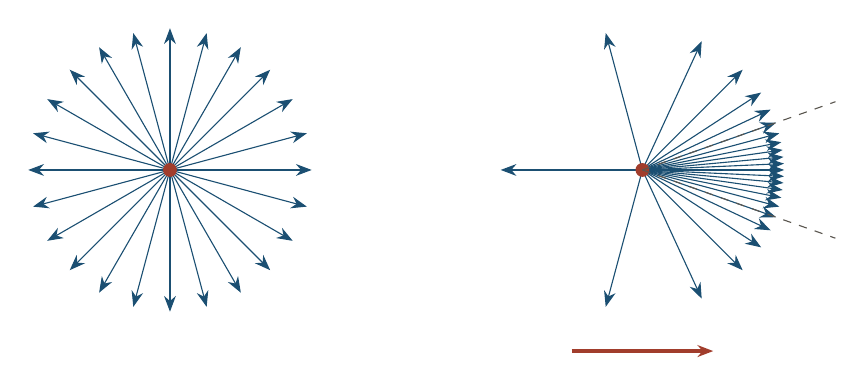
\begin{tikzpicture}[>={Stealth[length=2mm]}]
  \def\g{3}\pgfmathsetmacro{\b}{sqrt(1-1/(\g*\g))}
  \foreach \t in {0,15,...,345} { \draw[->, astroblue] (0,0) -- (\t:1.8); }
  \fill[accent] (0,0) circle (2.5pt);
  \begin{scope}[xshift=6cm]
    \foreach \t in {0,15,...,345} {
      \pgfmathsetmacro{\a}{atan2(sin(\t), \g*(cos(\t)+\b))}
      \draw[->, astroblue] (0,0) -- (\a:1.8);
    }
    \fill[accent] (0,0) circle (2.5pt);
    \draw[->, accent, line width=1.2pt] (-0.9,-2.3) -- (0.9,-2.3);
    \draw[dashed, muted] (0,0) -- ({atan(1/(\g*\b))}:2.6);
    \draw[dashed, muted] (0,0) -- ({-atan(1/(\g*\b))}:2.6);
  \end{scope}
\end{tikzpicture}
\end{document}
